%%%%%%%%%%%%%%%%%%%%%%%%%%%%%%%%%%%%%%%%%
% Dreuw & Deselaer's Poster
% LaTeX Template
% Version 1.0 (11/04/13)
%
% Created by:
% Philippe Dreuw and Thomas Deselaers
% http://www-i6.informatik.rwth-aachen.de/~dreuw/latexbeamerposter.php
%
% This template has been downloaded from:
% http://www.LaTeXTemplates.com
%
% License:
% CC BY-NC-SA 3.0 (http://creativecommons.org/licenses/by-nc-sa/3.0/)
%
%%%%%%%%%%%%%%%%%%%%%%%%%%%%%%%%%%%%%%%%%

%----------------------------------------------------------------------------------------
%	PACKAGES AND OTHER DOCUMENT CONFIGURATIONS
%----------------------------------------------------------------------------------------

\documentclass[final,hyperref={pdfpagelabels=false}]{beamer}

\usepackage[orientation=portrait,size=a0,scale=1.4]{beamerposter} % Use the beamerposter package for laying out the poster with a portrait orientation and an a0 paper size

\usetheme{I6pd2} % Use the I6pd2 theme supplied with this template

\usepackage[utf8]{inputenc}
\usepackage[brazil]{babel}

\usepackage{amsmath,amsthm,amssymb,latexsym} % For including math equations, theorems, symbols, etc

%\usepackage{times}\usefonttheme{professionalfonts}  % Uncomment to use Times as the main font
%\usefonttheme[onlymath]{serif} % Uncomment to use a Serif font within math environments

\boldmath % Use bold for everything within the math environment

\usepackage{booktabs} % Top and bottom rules for tables

\graphicspath{{figures/}} % Location of the graphics files

\usecaptiontemplate{\small\structure{\insertcaptionname~\insertcaptionnumber: }\insertcaption} % A fix for figure numbering

%----------------------------------------------------------------------------------------
%	TITLE SECTION
%----------------------------------------------------------------------------------------

\title{\huge Comunicação cliente-servidor bilateral de baixa latência aplicado a Android} % Poster title

\author{Guilherme Freire Silva, Marco Dimas Gubitoso (Orientador)} % Author(s)

\institute{IME-USP - Instituto de Matemática e Estatística da Universidade de São Paulo, Departamento de Ciência da Computação }
% \institute{Department and University Name} % Institution(s)

%----------------------------------------------------------------------------------------
%	FOOTER TEXT
%----------------------------------------------------------------------------------------

% \newcommand{\leftfoot}{http://www.LaTeXTemplates.com} % Left footer text
\newcommand{\leftfoot}{} % Left footer text

% \newcommand{\rightfoot}{john@smith.com} % Right footer text
\newcommand{\rightfoot}{} % Right footer text

%----------------------------------------------------------------------------------------

\begin{document}

\addtobeamertemplate{block end}{}{\vspace*{2ex}} % White space under blocks

\begin{frame}[t] % The whole poster is enclosed in one beamer frame

\begin{columns}[t] % The whole poster consists of two major columns, each of which can be subdivided further with another \begin{columns} block - the [t] argument aligns each column's content to the top

\begin{column}{.02\textwidth}\end{column} % Empty spacer column

\begin{column}{.465\textwidth} % The first column

%----------------------------------------------------------------------------------------
%	Introdução
%----------------------------------------------------------------------------------------

\begin{block}{Introdução}

\begin{itemize}
\item Dispositivos móveis, como smartphones e tables, são uma tecnologia muito nova e em constante desenvolvimento. Possuem bastante espaço para inovação, além de estarem fortemente presentes no dia a dia. Um aspecto pouco explorado deles é seu uso como parte de um sistema interativo Web, ou seja, um sistema no qual eles enviam e recebem informações de um servidor, para os mais variados fins.

\item Essa arquitetura permite, por exemplo, executar um jogo em uma página Web que utiliza o smartphone como um controle, ou manter um banco de dados no servidor e fazer buscas utilizando o smartphone.

\end{itemize}

\end{block}

%----------------------------------------------------------------------------------------
%	Objetivos
%----------------------------------------------------------------------------------------

\begin{block}{Objetivos}

\begin{enumerate}
\item Desenvolver um aplicativo para smartphones.
\item Criar um servidor que se comunique com ele.
\item Desenvolver uma aplicação Web que receba e utilize dados vindos do smartphone.
\item Encontrar uma forma eficiente de comunicação entre eles.
\end{enumerate}

\end{block}

%----------------------------------------------------------------------------------------
%	Aplicativo Mobile
%----------------------------------------------------------------------------------------

\begin{block}{Aplicativo Mobile}

\begin{columns} % Subdivide the first main column
\begin{column}{.54\textwidth} % The first subdivided column within the first main column

\begin{itemize}
\item Criado com o Framework Cordova.
\begin{itemize}
\item Multiplataforma, incluindo versão Web.
\end{itemize}
\item Conecta-se com o servidor através de um IP:Porta.
\begin{itemize}
\item Recebe e envia dados utilizando Sockets.
\end{itemize}
\end{itemize}

\begin{itemize}
\item Sobre sua interface e utilização.
\begin{itemize}
\item O formulário no início faz a conexão com o servidor, fornecidos o endereço de IP e a Porta.
\item Os botões azuis enviam mensagens pontuais ao servidor.
\item Os botões cinzas ligam ou desligam um fluxo de mensagens com dados do acelerômetro para o servidor.
\item O Log exibe mensagens vindas do servidor e outros feedbacks.
\end{itemize}
\end{itemize}

\end{column}

\begin{column}{.43\textwidth} % The second subdivided column within the first main column
\centering
\begin{figure}
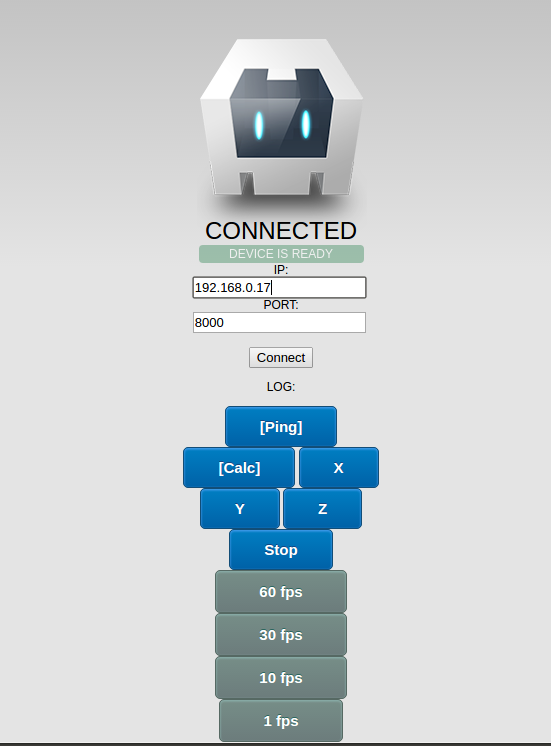
\includegraphics[width=0.8\linewidth]{Cordova.png}
\caption{Aplicativo Cordova}
\end{figure}
\end{column}
\end{columns} % End of the subdivision


\end{block}

%----------------------------------------------------------------------------------------
%	Comunicação
%----------------------------------------------------------------------------------------

\begin{block}{Comunicação utilizando Socket.io}

\begin{itemize}
\item Implementa o protocolo WebSocket.
\begin{itemize}
\item WebSocket lida com os sockets de uma conexão. Ele permite a comunicação bilateral por meio de uma interface simples.
\end{itemize}

\item Características do Socket.io:
\begin{itemize}
\item Orientado a eventos. Cada mensagem que chega é recebida como um evento. Se o processo escuta esse evento, ele executará uma função com os parâmetros recebidos.
\item Definição arbitrária de eventos. O código define quais eventos escuta e qual o evento que é enviado.
\item Assíncrono. Uma vez enviada a mensagem, o processo continua sua execução, sem precisar esperar um evento de resposta do outro processo.
\item Conexão bilateral. Pode enviar e receber mensagens livremente.
\item Baixa latência. O protocolo facilita ao máximo o envio e recebimento de mensagens.
\item Baixo \emph{overhead}. Possui um cabeçalho mínimo. Diferente de outros protocolos, ele possui somente o tipo de evento e o tamanho da mensagem enviada.
\item Permite multiplas conexões simultâneas. Através de multiplexação, permite que vários Sockets estejam conectados ao servidor através de uma única porta.
\item Se o servidor não permitir o uso de WebSockets, recorre a outras técnicas menos eficientes de comunicação bilateral, com a mesma interface.
\end{itemize}

\end{itemize}

\end{block}

%----------------------------------------------------------------------------------------

\end{column} % End of the first column

\begin{column}{.03\textwidth}\end{column} % Empty spacer column

\begin{column}{.465\textwidth} % The second column

%----------------------------------------------------------------------------------------
%	Server
%----------------------------------------------------------------------------------------

\begin{block}{Servidor}

\begin{itemize}
\item Escrito em JavaScript com ajuda de Node.js e ExpressJS.
\item Fornece a página HTML que executa o código da aplicação.
\item Com a utilização de Socket.io, aceita a conexão com o smartphone.
\begin{itemize}
\item Permite a conexão com múltiplos dispositivos simultaneamente.
\end{itemize}
\item Recebe eventos do smartphone e o responde ou repassa esses dados à página Web.
\end{itemize}

\end{block}

%----------------------------------------------------------------------------------------
%	Página Web
%----------------------------------------------------------------------------------------

\begin{block}{Exemplo simples de Aplicação Web - Esfera Interativa}

\begin{columns} % Subdivide the first main column
\begin{column}{.54\textwidth} % The first subdivided column within the first main column

\begin{itemize}
\item Utiliza a biblioteca 3D para JavaScript THREE.js.
\begin{itemize}
\item Utiliza a GPU do usuário para renderizar o cenário 3D.
\end{itemize}
\item Mantém um socket aberto para a conexão com o servidor.
\item Inicia-se estática, mas recebe eventos para aumentar e reduzir sua velocidade nos eixos X, Y e Z.
\item Pode receber um outro evento, que chega a intervalos constantes e define sua velocidade de acordo com o acelerômetro do smartphone.
\begin{itemize}
\item Esse evento explicita a baixa lantência alcançada com o uso de Socket.io para a comunicação, pois é um feedback quase instantâneo à movimentação do dispositivo pelo usuário.
\end{itemize}
\end{itemize}

% \begin{itemize}
% \item Sobre sua interface e utilização.
% \begin{itemize}
% \item O formulário no início faz a conexão com o servidor, fornecidos o endereço de IP e a Porta.
% \end{itemize}
% \end{itemize}

\end{column}

\begin{column}{.43\textwidth} % The second subdivided column within the first main column
\centering
\begin{figure}
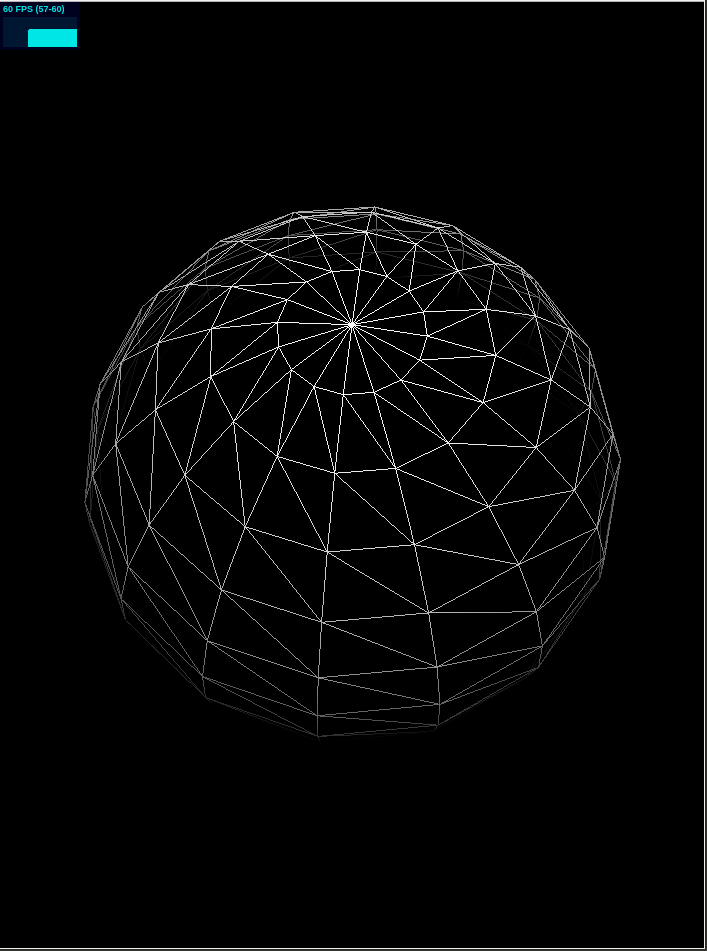
\includegraphics[width=0.8\linewidth]{sphere.png}
\caption{Esfera interativa}
\end{figure}
\end{column}
\end{columns} % End of the subdivision

\end{block}

%------------------------------------------------

% \begin{block}{Results: Figure}

% \begin{figure}
% 
\includegraphics[width=0.8\linewidth]{placeholder.jpg}
% \caption{Figure caption}
% \end{figure}

% \end{block}

%----------------------------------------------------------------------------------------
%	CONCLUSION
%----------------------------------------------------------------------------------------

\begin{block}{Conclusão}

\begin{itemize}
\item O projeto proposto se mostrou plenamente possível e viável, com a utilização das ferramentas certas.
\item As aplicações desenvolvidas e apresentadas possuem os elementos básicos para a criação de sistemas muito maiores a mais robustos.
\item Em resumo, foi criado um arcabouço para a comunicação bilateral entre múltiplos clientes e um servidor, esses clientes podendo ser executados em smartphones, tirando proveito de suas funcionalidades exclusivas.
\end{itemize}

\end{block}

%----------------------------------------------------------------------------------------
%	REFERENCES
%----------------------------------------------------------------------------------------

\begin{block}{Referências}

\begin{thebibliography}{99}

\bibitem{ac} Socket.io,
\textit{http://socket.io/}

\bibitem{ac} WebSocket,
\textit{http://websocket.org/}

\bibitem{ac} Apache Cordova,
\textit{https://cordova.apache.org/}

\bibitem{ac} Node.JS,
\textit{https://nodejs.org/en/}

\bibitem{tj} THREE.js,
\textit{https://threejs.org/}

\end{thebibliography}
\end{block}


%----------------------------------------------------------------------------------------
%	IMAGEM
%----------------------------------------------------------------------------------------

\begin{block}{}

\begin{figure}

\includegraphics[width=0.3\linewidth]{logoIME.png}
\end{figure}

\end{block}

%----------------------------------------------------------------------------------------
%	ACKNOWLEDGEMENTS
%----------------------------------------------------------------------------------------

% \begin{block}{Acknowledgments}

% \begin{itemize}
% \item Nam mollis tristique neque eu luctus. Suspendisse rutrum congue nisi sed convallis. Aenean id neque dolor. Pellentesque habitant morbi tristique senectus et netus et malesuada fames ac turpis egestas.
% \end{itemize}

% \end{block}

%----------------------------------------------------------------------------------------
%	CONTACT INFORMATION
%----------------------------------------------------------------------------------------

% \setbeamercolor{block title}{fg=black,bg=orange!70} % Change the block title color

% \begin{block}{Contact Information}

% \begin{itemize}
% \item Web: \href{http://www.university.edu/smithlab}{http://www.university.edu/smithlab}
% \item Email: \href{mailto:john@smith.com}{john@smith.com}
% \item Phone: +1 (000) 111 1111
% \end{itemize}

% \end{block}

%----------------------------------------------------------------------------------------

\end{column} % End of the second column

\begin{column}{.015\textwidth}\end{column} % Empty spacer column

\end{columns} % End of all the columns in the poster

\end{frame} % End of the enclosing frame

\end{document}